\mySection{12.3 Multiple Comparisons: Turkey's Method}
%-------------- start slide -------------------------------%{{{ 12.51
\begin{frame}
	% {\S\: 12.3 Multiple Comparisons: Turkey's Method}
\begin{center}
	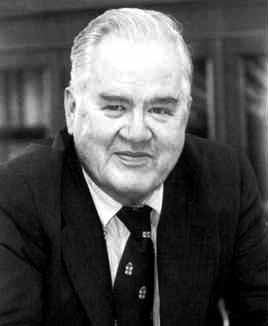
\includegraphics[scale=0.25]{John_Tukey.jpg} \\[2em]
	\small
	\begin{enumerate}
	\item John Wilder Tukey (June 16, 1915 -- July 26, 2000)
		was an American mathematician best known for
		development of the Fast Fourier Transform (FFT) algorithm and box plot.
	\item The Tukey range test, the Tukey lambda distribution,
		the Tukey test of additivity,
		and the Teichm\"uller-Tukey lemma all bear his name.
	\item  He is also credited with coining the term 'bit'.
	\end{enumerate}
	\vfill
	\url{https://en.wikipedia.org/wiki/John_Tukey}
	\end{center}
\end{frame}
%-------------- end slide -------------------------------%}}}
%-------------- start slide -------------------------------%{{{ 12.52
\begin{frame}[fragile]

	\begin{enumerate}
		\item[]
	\begin{center}
		\begin{tabular}{cccc}
			$N(\mu_1,\sigma^2)$ & $N(\mu_2,\sigma^2)$ & $\cdots$ & $N(\mu_2,\sigma^2)$ \\
			\hline
			$Y_{11}$ & $Y_{12}$ & $\cdots$ & $Y_{1k}$\cr
			$Y_{21}$ & $Y_{22}$ & $\cdots$ & $Y_{2k}$\cr
			$\vdots$ & $\vdots$ & $\vdots$ & $\vdots$\cr
			$Y_{r1}$ & $Y_{r2}$ & $\cdots$ & $Y_{rk}$\cr
			\hline
		\end{tabular}
	\end{center}
	\vfill
\item[Goal] For any $i\ne j$, test
	\[
	H_0: \mu_i =\mu_j \qquad v.s. \qquad H_1: \mu_i\ne \mu_j
	\]
	\vfill
\item[] at the $\alpha$ level of significance defined as
	\[
		\bbP \left(\bigcup_{j=1}^{{k\choose 2}}E_j\right) = \alpha
	\]
\item[] where there are ${k\choose 2}$ pairs, and $E_j$ is the event of making a type I error for the $j$-th pair.
	\end{enumerate}

\end{frame}
%-------------- end slide -------------------------------%}}}
%-------------- start slide -------------------------------%{{{ 12.53
\begin{frame}[fragile]
\begin{enumerate}
	\item[Goal'] Simultaneous C.I.'s for ${k\choose 2}$ pairs of means:
	\item[] Given $\alpha$, find $I_{ij}$, the C.I. for $\mu_i-\mu_j$ (with $i,j=1,\cdots,k$ and $i\ne j$), s.t.
	\item[]
		\[
			\bbP\left(\mu_i-\mu_j\in I_{ij},\: \forall i,j=1,\cdots, k, i\ne j\right) = 1-\alpha.
		\]
\end{enumerate}

\end{frame}
%-------------- end slide -------------------------------%}}}
%-------------- start slide -------------------------------%{{{ 12.54
\begin{frame}[fragile]

	\begin{enumerate}
		\item[???] Why not the standard pair-wise two-sample t-test?
		\item[] Suppose $\bbP(E_j)=\alpha_*$. Then
			\begin{align*}
\alpha & = \bbP \left(\bigcup_{j=1}^{{k\choose 2}}E_j\right)
= 1-  \bbP \left(\bigcap_{j=1}^{{k\choose 2}}E_j^c \right)
\approx 1- \prod_{j=1}^{k\choose 2} \bbP(E_j^c)
= 1-(1-\alpha_*)^{k\choose 2}
			\end{align*}
		\item[] Hence,
		\[
			\alpha_* \approx  1-(1-\alpha)^{1/{k\choose 2}}
		\]
		\vfill
	\item[] E.g., $\alpha=0.05$
		\begin{center}
			\begin{tabular}{c|ccc}
				$k$ & 5 & 8 & 100 \\
				\hline
				$\alpha_*$ & 0.0051162 & 0.001830 & 0.00001036
			\end{tabular}
		\end{center}
	\end{enumerate}
\end{frame}
%-------------- end slide -------------------------------%}}}
%-------------- start slide -------------------------------%{{{ 12.55
\begin{frame}[fragile]{Bonferroni's method \\
		\small --- A straightforward method}
		\begin{minipage}{0.4\textwidth}
	\begin{enumerate}
		\item[]
			\begin{align*}
				\bbP\left(\mu_i-\mu_j\in I_{ij},\: \forall i\ne j\right)
			\end{align*}
		\item[]
			\[||\]
			\[
			\bbP\left(\bigcap_{i\ne j}\mu_i-\mu_j\in I_{ij}\right)
			\]
		\item[]
			\[||\]
			\[
				1-\bbP\left(\bigcup_{i\ne j}\mu_i-\mu_j\not\in I_{ij}\right)
			\]
		\item[]
			\[\text{\rotatebox[origin=c]{90}{$\le$}}\]
			\[
				1-\sum_{i\ne j} \bbP\left(\mu_i-\mu_j\not\in I_{ij}\right)
			\]
		\item[]
			\[||\]
			\[
				1 - {k\choose 2} \alpha_*
			\]
	\end{enumerate}
		\end{minipage}
		\hfill\pause
		\begin{minipage}{0.55\textwidth}
			\begin{enumerate}
				\item
			 If we choose $\alpha_* = \alpha/{k\choose 2}$,
		 \item let $I_{ij}$ be the $(1-\alpha_*)100\%$ C.I. $i\ne j$
		 \item[]
			 \[\Downarrow\]
			\begin{align*}
				\bbP\left(\mu_i-\mu_j\in I_{ij},\: \forall i\ne j\right)
			\end{align*}
			\[\text{\rotatebox[origin=c]{90}{$\le$}}\]
			\[
				1 - {k\choose 2} \alpha_*
			\]
			\[||\]
			\[
			1-\alpha.
			\]
			\end{enumerate}
		\end{minipage}
\end{frame}
%-------------- end slide -------------------------------%}}}
%-------------- start slide -------------------------------%{{{ 12.56
\begin{frame}[fragile]

	\begin{enumerate}
\item[Remark] This is an approximation. The resulting C.I. are in general too wide.\\[1em]
\item[] The exact, and much more precise, solution is given by J.W. Turkey.\\[1em]
\item[] One can also construct simultaneous C.I. for all possible linear combinations of the parameters $\sum_{j=1}^k c_j \mu_j$, this can be acchieved by {\bf Scheff\'e's method}. A simple verson is given in \S 12.4.
	\end{enumerate}
\end{frame}
%-------------- end slide -------------------------------%}}}
%-------------- start slide -------------------------------%{{{ 12.57
\begin{frame}[fragile]{Tukey's HSD (honestly significant difference) test}
	\begin{enumerate}
		\item[] Let's construct $(1-\alpha)100\%$ C.I.'s simultaneously for all pairs.
			\vfill
		\item[]
			\[
				\bbP\left(\left|(\overline{Y}_{\cdot i}-\mu_i) - (\overline{Y}_{\cdot j}-\mu_j)\right|\le \mathcal{E},\quad \forall i\ne j\right) = 1-\alpha
			\]
		\item[]
			\[
				||
			\]
			\[
				\bbP\left(\max_{i}(\overline{Y}_{\cdot i}-\mu_i) - \min_{j}(\overline{Y}_{\cdot j}-\mu_j)\le \mathcal{E}\right)\hspace{3em}
			\]
		\item[]
			\[
				||
			\]
			\[
				\bbP\left(\max_{i}\overline{Y}_{\cdot i} - \min_{j}\overline{Y}_{\cdot j}\le \mathcal{E}\right)\hspace{3em}
			\]
			\vfill
		\item[$\Longrightarrow$]  Needs to study  ...
	\end{enumerate}
\end{frame}
%-------------- end slide -------------------------------%}}}
%-------------- start slide -------------------------------%{{{ 12.58
\begin{frame}[fragile]

	\begin{enumerate}
		\item[Def.] Let $W_1,\cdots, W_k$ be $k$ i.i.d. r.v.'s from $N(\mu,\sigma^2)$. Let $R$ denote their range:
		\[
		R =\max_i W_ i -\min_i W_i.
		\]
		Let $S^2$ be an unbiased estimator for $\sigma^2$ independent of the $W_i$'s and based on $\nu$ df.
		Define the {\bf Studentized range, $Q_{k,\nu}$}, to be the ratio:
		\[
			Q_{k,\nu} :=\frac RS.
		\]
		\vfill
	\item[]
		\begin{center}
			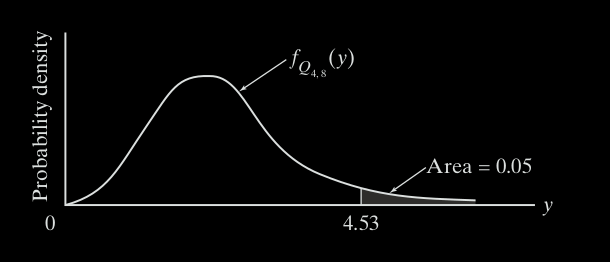
\includegraphics[scale=0.35]{Figure_12-3-1-neg.png}
		\end{center}
	\item[Remark]
		\begin{enumerate}
			\item We need $R\perp S$ to mimic Student's t-distribution.
			\item In the following $\nu = n-k = rk -k = r(k-1)$.
		\end{enumerate}
\end{enumerate}
\end{frame}
%-------------- end slide -------------------------------%}}}
%-------------- start slide -------------------------------%{{{ 12.59
\begin{frame}[fragile]
	\begin{center}

		\begin{enumerate}
			\item[] $Q_{k,\nu}\sim$ {\bf Studentized range distribution} with parameters $k$ and $\nu$.
			\item[] $k$: number of groups.
			\item[] $\nu$: degrees of freedom.
				\vfill
			\item[]
		\end{enumerate}
		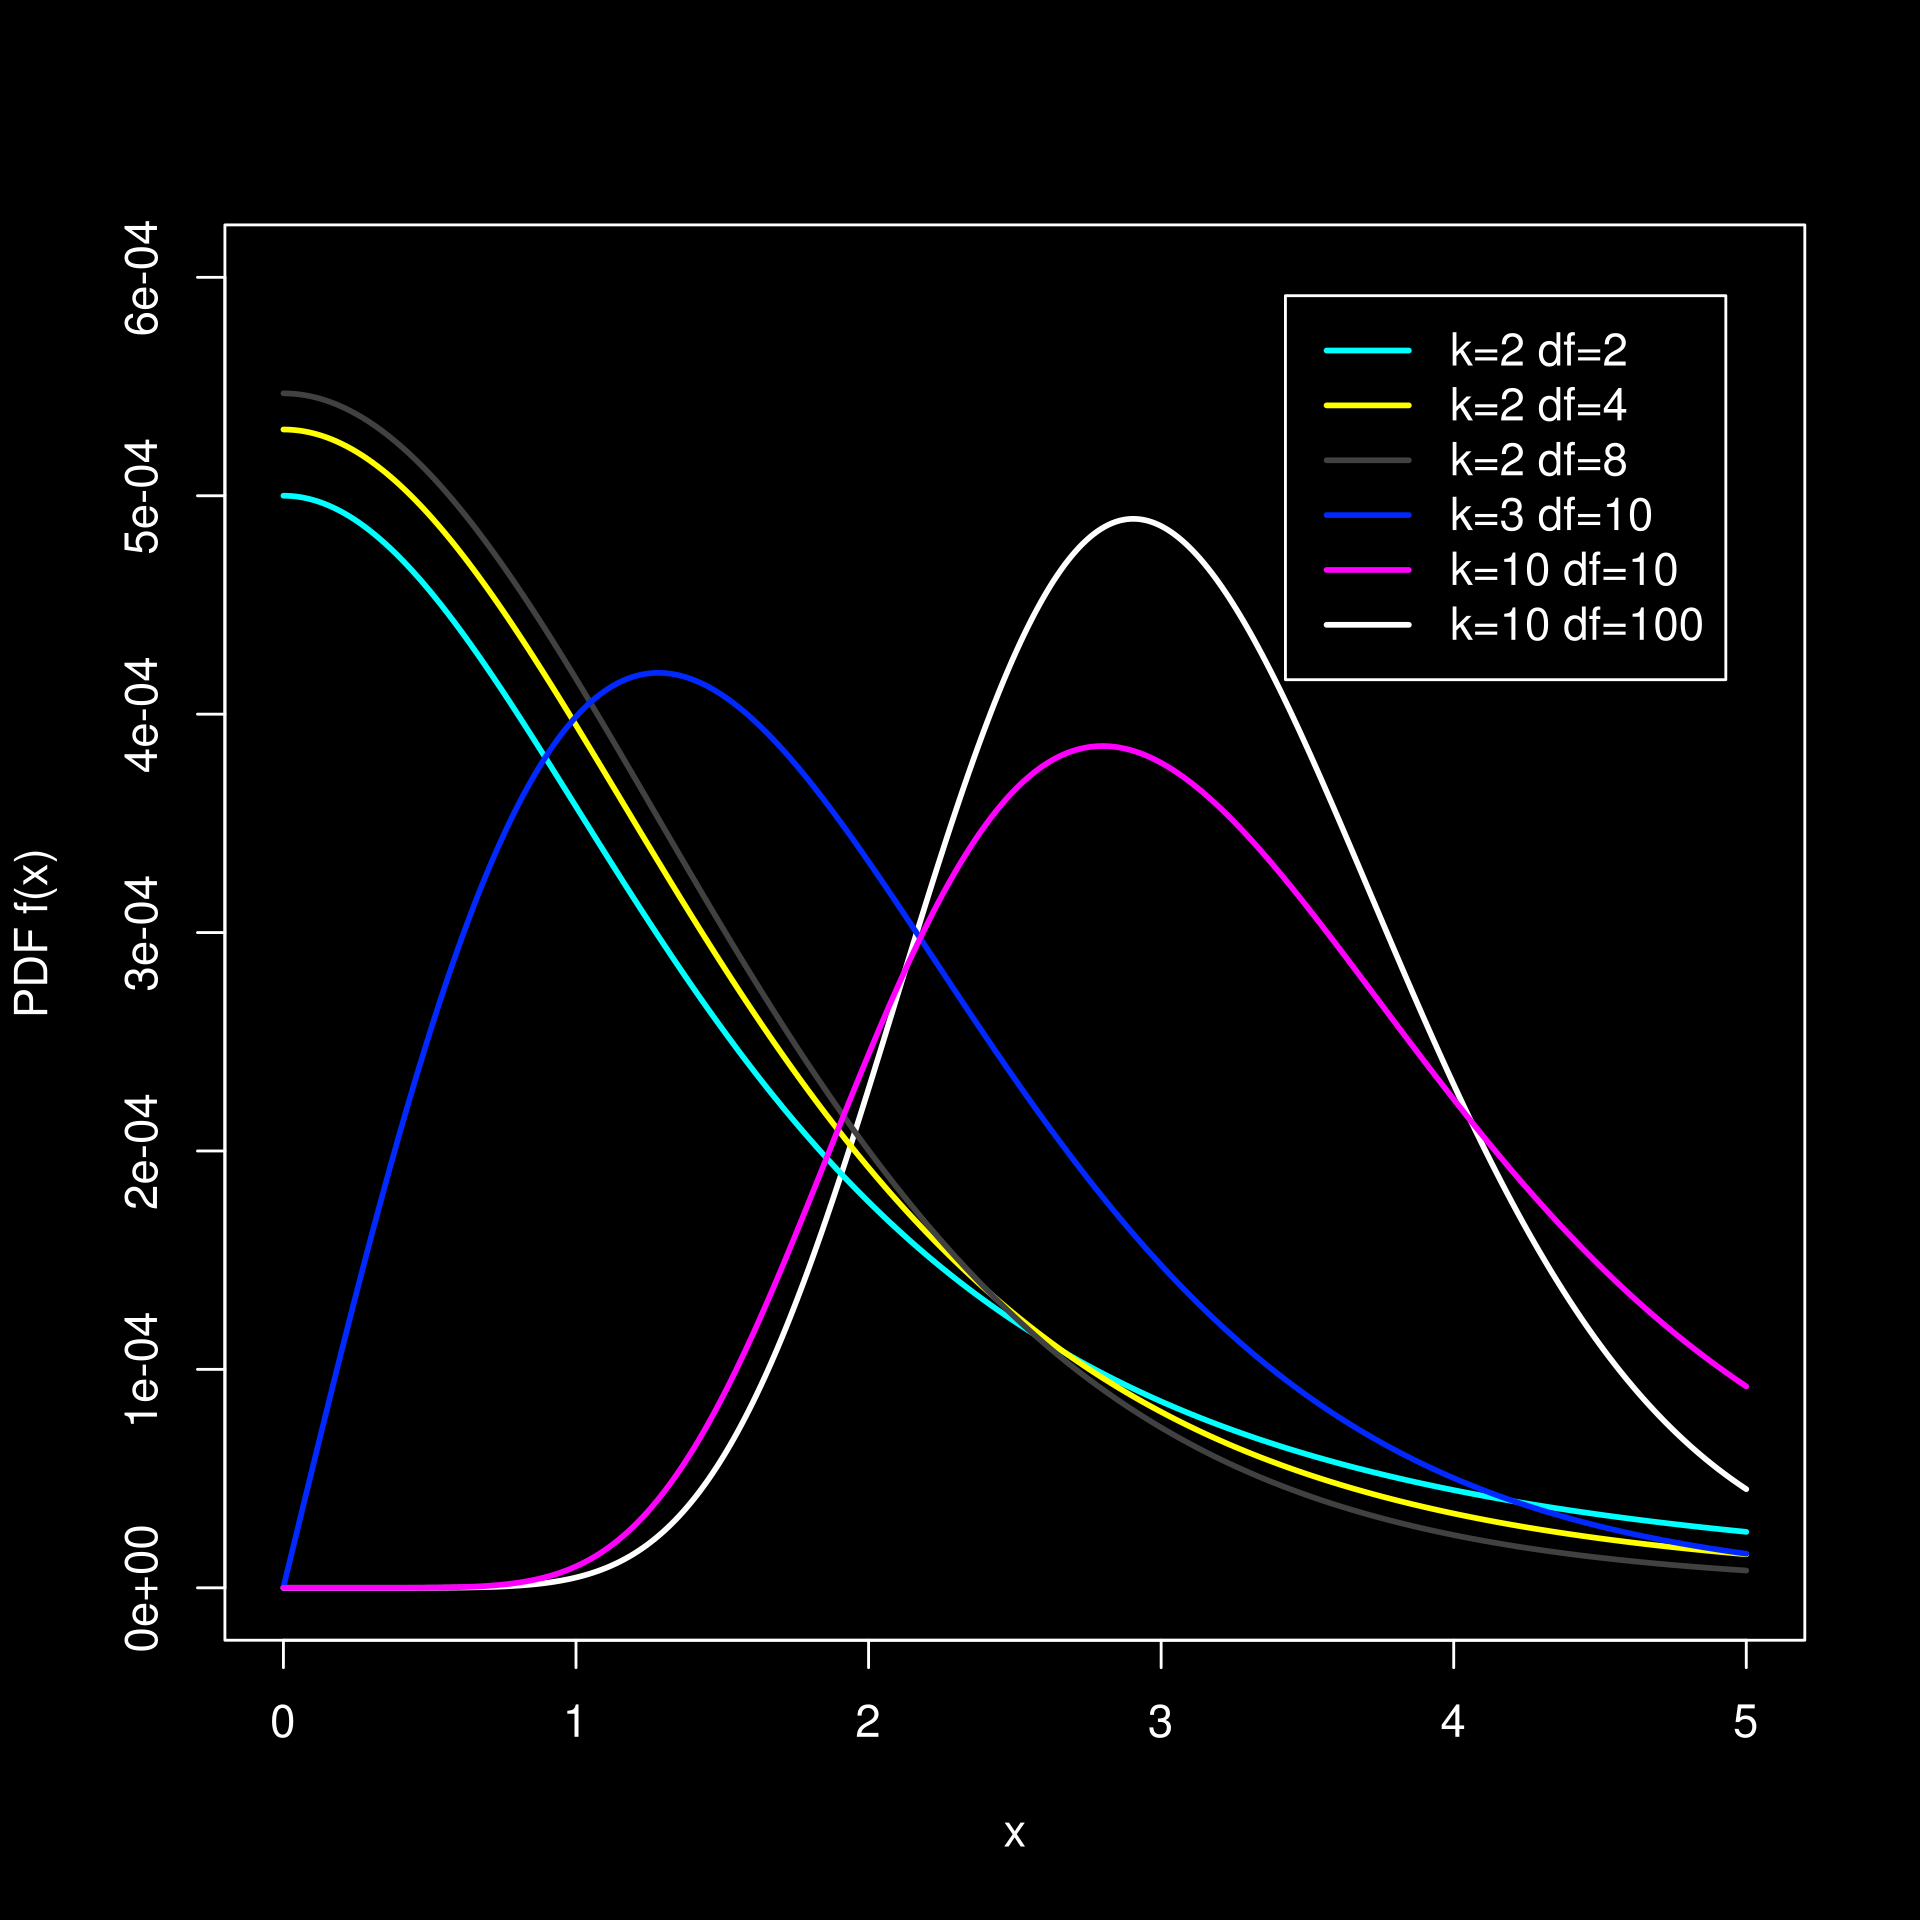
\includegraphics[scale=0.1]{1920px-StudentizedRangePDF.svg-neg.png}
	\end{center}
\end{frame}
%-------------- end slide -------------------------------%}}}
%-------------- start slide -------------------------------%{{{ 12.60
\begin{frame}[fragile]
	Let's find one example that all requirements of the $Q_{k,\nu}$ are satisfied.
	\vfill
	\begin{enumerate}
		\item Take $W_j = \overline{Y}_{\cdot j}-\mu_j$, $j=1,\cdots,k$ $\quad\Longrightarrow\quad$ $W_j\sim N(0,\sigma^2/r)$.
			\vfill
		\item $MSE$ or the pooled variance $S_p^2$ \hfill $MSE/r$
		\item[] \qquad is an unbiased estimator for $\sigma^2$ \hfill $\sigma^2/r$
		\item[] \qquad is $\perp\{\overline{Y}_{\cdot j}\}_{j=1,\cdots, k}$, hence $\perp\{W_j\}_{j=1,\cdots, k}$
			\vfill
		\item $df$ of $MSE$ is equal to $n-k=kr-k = k(r-1)$.
			\vfill
		\item[$\Longrightarrow$] \hspace{1em} $\displaystyle \frac{\max_{i}W_i - \min_j W_j}{\sqrt{MSE/r}} \sim $ Studentized range distribution($k$, $rk-k$)
	\end{enumerate}
\end{frame}
%-------------- end slide -------------------------------%}}}
%-------------- start slide -------------------------------%{{{ 12.61
\begin{frame}[fragile]

	\begin{enumerate}
		\item[]
	\[
		\hspace{3em}		\bbP \left( \frac{\max_{i}W_i - \min_j W_j}{\sqrt{MSE/r}} \le Q_{\alpha,k,rk-k}  \right ) = 1-\alpha
	\]
		\item[]
	\[||\]
	\[
		\bbP \left(\max_i W_i -\min_j W_j \le \frac{Q_{\alpha,k,rk-k}}{\sqrt{r}}\sqrt{MSE}\right)
	\]
		\item[]
	\[||\]
	\[
		\bbP \left(\left| W_i -W_j\right| \le \frac{Q_{\alpha,k,rk-k}}{\sqrt{r}}\sqrt{MSE},\:\:\forall i\ne j\right)
	\]
		\item[]
	\[||\]
	\[
		\bbP \left(\left| \left(\overline{Y}_{\cdot i} -\overline{Y}_{\cdot j}\right) - (\mu_i-\mu_j)\right| \le \frac{Q_{\alpha,k,rk-k}}{\sqrt{r}}\sqrt{MSE},\:\:\forall i\ne j\right)
	\]
		\item[]
	\[||\]
	\[
		\hspace{-2em}		\bbP \left(
			\overline{Y}_{\cdot i} -\overline{Y}_{\cdot j} - \frac{Q_{\alpha,k,rk-k}}{\sqrt{r}}\sqrt{MSE}
		\le \mu_i-\mu_j \le
			\overline{Y}_{\cdot i} -\overline{Y}_{\cdot j}+ \frac{Q_{\alpha,k,rk-k}}{\sqrt{r}}\sqrt{MSE}
		,\:\: \forall i\ne j\right )
	\]
	\end{enumerate}
\end{frame}
%-------------- end slide -------------------------------%}}}
%-------------- start slide -------------------------------%{{{ 12.62
\begin{frame}[fragile]

	\begin{enumerate}
		\item[] Therefore, for all $i\ne j$,
			the $100(1-\alpha)\%$ C.I. for $ \mu_i-\mu_j $ is \\[2em]
			\[
			\overline{Y}_{\cdot i} -\overline{Y}_{\cdot j} \pm  \frac{Q_{\alpha,k,rk-k}}{\sqrt{2}}\sqrt{MSE}\sqrt{\frac 2r}
			\]
			\vfill
		\item[] To test $H_0: \mu_i=\mu_j$ for specific $i\ne j$, reject $H_0$ in favor of $H_1:\mu_i\ne\mu_j$ if the C.I. does NOT contain $0$, at the $\alpha$ level of significance.\myEnd
			\vfill
		\item[Note:] When sample sizes are not equal, use the {\bf Tukey-Kramer method}: \\[2em]
			\[
				\overline{Y}_{\cdot i} -\overline{Y}_{\cdot j} \pm  \frac{Q_{\alpha,k,rk-k}}{\sqrt{2}}\sqrt{MSE}\sqrt{\frac{1}{r_i} + \frac{1}{r_j}}
			\]
	\end{enumerate}
\end{frame}
%-------------- end slide -------------------------------%}}}
%-------------- start slide -------------------------------%{{{ 12.63
\begin{frame}
	\begin{enumerate}
		\item[E.g. 2] A certain fraction of antibiotics injected into the bloodstream are ``bound'' to
serum proteins. This phenomenon bears directly on the effectiveness of the
medication, because the binding decreases the systemic uptake of the drug.
Table below lists the binding percentages in bovine serum measured for five
widely prescribed antibiotics. Which antibiotics have similar binding
properties, and which are different? \\[1em]
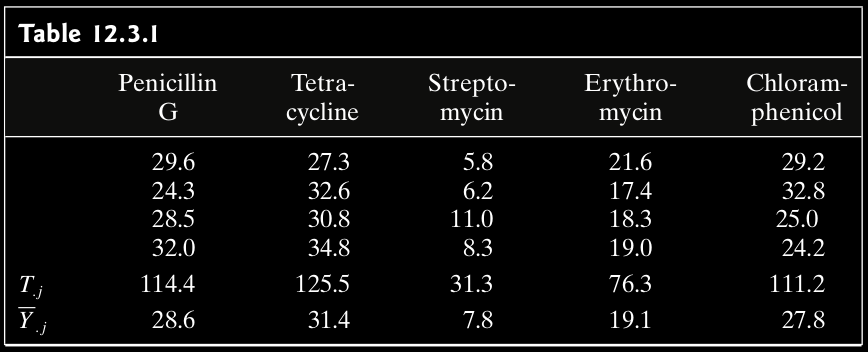
\includegraphics[scale=0.25]{Table_12-3-1-neg.png}
	\end{enumerate}
\end{frame}
%-------------- end slide -------------------------------%}}}
%-------------- start slide -------------------------------%{{{ 12.64
\begin{frame}[fragile]
	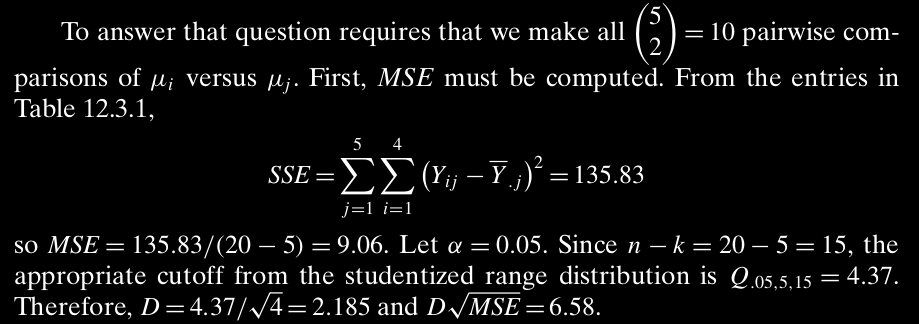
\includegraphics[scale=0.28]{Case_12-3-1-Sol1-neg.png}\\
	\vfill
	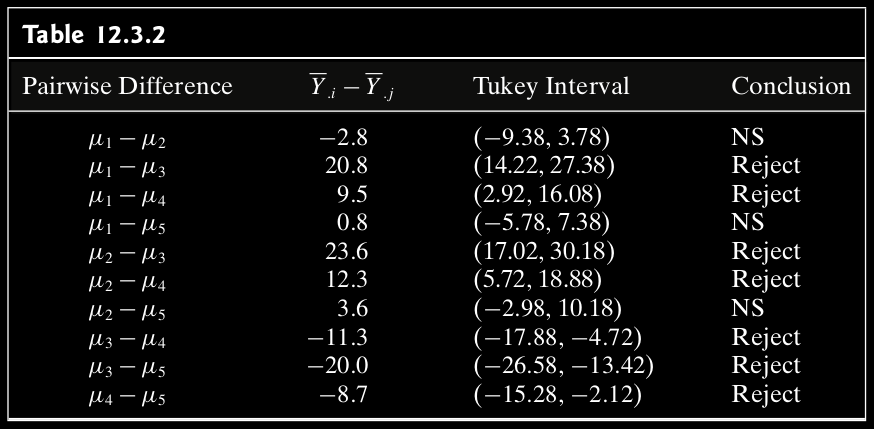
\includegraphics[scale=0.3]{Table_12-3-2-neg.png}
\end{frame}
%-------------- end slide -------------------------------%}}}
%-------------- start slide -------------------------------%{{{ 12.65
\begin{frame}[fragile]
	\begin{minipage}{0.3\textwidth}
	\begin{lstlisting}
> # Case Study 12.3.1
> # Input data first
> Input <- c("
+ rates group
+ 29.6  M1
+ 24.3  M1
+ 28.5  M1
+ 32.0  M1
+ 27.3  M2
+ 32.6  M2
+ 30.8  M2
+ 34.8  M2
+ 5.8   M3
+ 6.2   M3
+ 11.0  M3
+ 8.3   M3
+ 21.6  M4
+ 17.4  M4
+ 18.3  M4
+ 19.0  M4
+ 29.2  M5
+ 32.8  M5
+ 25.0  M5
+ 24.2 M5
+ ")
> Data = read.table(
 	textConnection(Input),
+       header=TRUE)
	\end{lstlisting}
	\end{minipage}
	\begin{minipage}{0.63\textwidth}
	\begin{lstlisting}
> # Compute one-way ANOVA test
> res.aov <- aov(rates ~ group, data = Data)
> # Summary of the analysis
> summary(res.aov)
            Df Sum Sq Mean Sq F value   Pr(>F)
group        4 1480.8   370.2   40.88 6.74e-08 ***
Residuals   15  135.8     9.1
---
Signif. codes:  0 '***' 0.001 '**' 0.01 '*' 0.05 '.' 0.1 ' ' 1
	\end{lstlisting}
	\end{minipage}

\end{frame}
%-------------- end slide -------------------------------%}}}
%-------------- start slide -------------------------------%{{{ 12.66
\begin{frame}[fragile]
	\begin{center}
		\begin{minipage}{0.6\textwidth}
	\begin{lstlisting}
> # Tukey multiple pairwise-comparisons
> TukeyHSD(res.aov)
  Tukey multiple comparisons of means
    95% family-wise confidence level

Fit: aov(formula = rates ~ group, data = Data)

$group
         diff        lwr        upr     p adj
M2-M1   2.775  -3.795401   9.345401 0.6928357
M3-M1 -20.775 -27.345401 -14.204599 0.0000006
M4-M1  -9.525 -16.095401  -2.954599 0.0034588
M5-M1  -0.800  -7.370401   5.770401 0.9952758
M3-M2 -23.550 -30.120401 -16.979599 0.0000001
M4-M2 -12.300 -18.870401  -5.729599 0.0003007
M5-M2  -3.575 -10.145401   2.995401 0.4737713
M4-M3  11.250   4.679599  17.820401 0.0007429
M5-M3  19.975  13.404599  26.545401 0.0000010
M5-M4   8.725   2.154599  15.295401 0.0071611
	\end{lstlisting}
		\end{minipage}
	\end{center}
\end{frame}
%-------------- end slide -------------------------------%}}}
%-------------- start slide -------------------------------%{{{ 12.67
\begin{frame}[fragile]
	\begin{center}
		\begin{minipage}{0.6\textwidth}
	\begin{lstlisting}
> round(TukeyHSD(res.aov)$group,2)
					diff   		 lwr		    upr		 p adj
M2-M1		   2.78		  -3.80		   9.35		  0.69
M3-M1		 -20.77		 -27.35		 -14.20		  0.00
M4-M1		  -9.52		 -16.10		  -2.95		  0.00
M5-M1		  -0.80		  -7.37		   5.77		  1.00
M3-M2		 -23.55		 -30.12		 -16.98		  0.00
M4-M2		 -12.30		 -18.87		  -5.73		  0.00
M5-M2		  -3.58		 -10.15		   3.00		  0.47
M4-M3		  11.25		   4.68		  17.82		  0.00
M5-M3		  19.97		  13.40		  26.55		  0.00
M5-M4		   8.73		   2.15		  15.30		  0.01
---
Signif. codes:  0 '***' 0.001 '**' 0.01 '*' 0.05 '.' 0.1 ' ' 1
(Adjusted p values reported -- single-step method)
	\end{lstlisting}
		\end{minipage}
		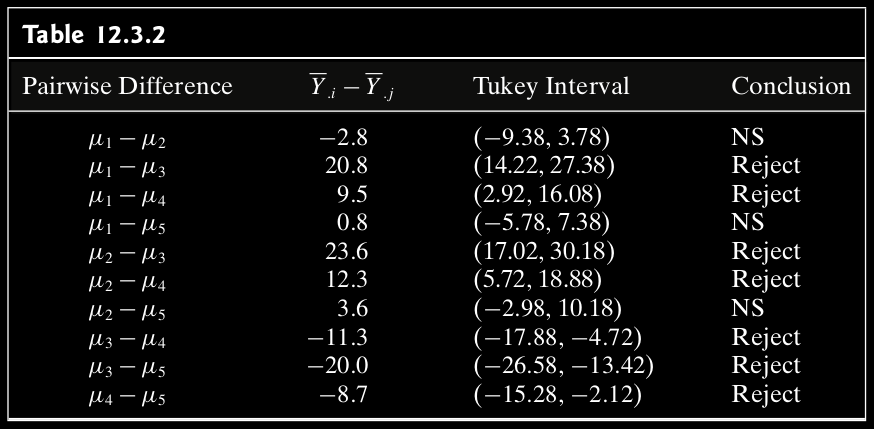
\includegraphics[scale=0.25]{Table_12-3-2-neg.png}
	\end{center}
\end{frame}
%-------------- end slide -------------------------------%}}}
%-------------- start slide -------------------------------%{{{ 12.68
\begin{frame}[fragile]
	\begin{center}
		\begin{minipage}{0.7\textwidth}
	\begin{lstlisting}
	> # Or one may use multcomp package or multiple comparisons
> library(multcomp)
> summary(glht(res.aov, linfct = mcp(group = "Tukey")))

	 Simultaneous Tests for General Linear Hypotheses

Multiple Comparisons of Means: Tukey Contrasts


Fit: aov(formula = rates ~ group, data = Data)

Linear Hypotheses:
             Estimate Std. Error t value Pr(>|t|)
M2 - M1 == 0    2.775      2.128   1.304  0.69283
M3 - M1 == 0  -20.775      2.128  -9.764  < 0.001 ***
M4 - M1 == 0   -9.525      2.128  -4.477  0.00348 **
M5 - M1 == 0   -0.800      2.128  -0.376  0.99528
M3 - M2 == 0  -23.550      2.128 -11.068  < 0.001 ***
M4 - M2 == 0  -12.300      2.128  -5.781  < 0.001 ***
M5 - M2 == 0   -3.575      2.128  -1.680  0.47374
M4 - M3 == 0   11.250      2.128   5.287  < 0.001 ***
M5 - M3 == 0   19.975      2.128   9.388  < 0.001 ***
M5 - M4 == 0    8.725      2.128   4.101  0.00717 **
---
Signif. codes:  0 '***' 0.001 '**' 0.01 '*' 0.05 '.' 0.1 ' ' 1
(Adjusted p values reported -- single-step method)
	\end{lstlisting}
		\end{minipage}
	\end{center}
\end{frame}
%-------------- end slide -------------------------------%}}}
%-------------- start slide -------------------------------%{{{ 12.69
\begin{frame}[fragile]
	\begin{center}
		\begin{minipage}{0.7\textwidth}
	\begin{lstlisting}
	             Estimate Std. Error t value Pr(>|t|)
M2 - M1 == 0    2.775      2.128   1.304  0.69283
M3 - M1 == 0  -20.775      2.128  -9.764  < 0.001 ***
M4 - M1 == 0   -9.525      2.128  -4.477  0.00348 **
M5 - M1 == 0   -0.800      2.128  -0.376  0.99527
M3 - M2 == 0  -23.550      2.128 -11.068  < 0.001 ***
M4 - M2 == 0  -12.300      2.128  -5.781  < 0.001 ***
M5 - M2 == 0   -3.575      2.128  -1.680  0.47371
M4 - M3 == 0   11.250      2.128   5.287  < 0.001 ***
M5 - M3 == 0   19.975      2.128   9.388  < 0.001 ***
M5 - M4 == 0    8.725      2.128   4.101  0.00719 **
	\end{lstlisting}
		\end{minipage}
		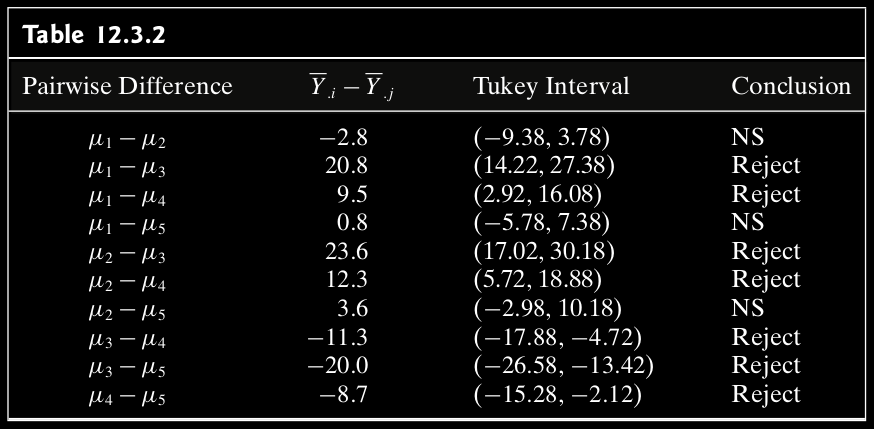
\includegraphics[scale=0.25]{Table_12-3-2-neg.png}
	\end{center}
\end{frame}
%-------------- end slide -------------------------------%}}}
%-------------- start slide -------------------------------%{{{ 12.70
\begin{frame}{Two more examples of ANOVA using R}
	\begin{enumerate}
		\item[E.g. 1] \url{http://www.sthda.com/english/wiki/one-way-anova-test-in-r}
			\vfill
		\item[E.g. 2] \url{https://datascienceplus.com/one-way-anova-in-r/}
	\end{enumerate}
\end{frame}
%-------------- end slide -------------------------------%}}}
